\documentclass[10pt,a4paper]{article}
\usepackage[margin=16mm]{geometry}
\usepackage[T1]{fontenc}
\usepackage{lmodern,amsmath,amssymb,booktabs,array,graphicx,enumitem}
\usepackage[hidelinks]{hyperref}
\usepackage{microtype}
\graphicspath{{./}}
\setlength{\parindent}{0pt}
\setlength{\parskip}{4pt}
\setlist{nosep,leftmargin=18pt}
\newcommand{\R}{\mathbb{R}}
\newcommand{\E}{\mathbb{E}}
\newcommand{\ind}{\mathbf{1}}
\newcommand{\softmax}{\operatorname{softmax}}
\newcommand{\sigmoid}{\operatorname{sigmoid}}
\newcommand{\softplus}{\operatorname{softplus}}
\title{Foundations of TRAC-Engage\\\large From neural networks to continuous, track-aware engagement estimation}
\author{Companion mathematical notes to the revised architecture proposal}
\date{14 October 2026}
\begin{document}
\maketitle
\vspace{-6mm}
\textbf{Prerequisites.} Neural networks as function approximators, convolution, recurrent networks, attention and a Transformer block. These notes derive the additional concepts needed to understand and implement the proposed system. They distinguish the complete research design from the smaller software implementation currently available. They do not present a trained production detector.

\section{What function are we trying to learn?}
Let $I_t\in\R^{H\times W\times3}$ be a video frame at event time $t$. An ordinary classifier approximates $f_\theta(x)\approx y$. Here the input is not one image and the answer is not one label for the whole scene. We need a set of person-specific outputs:
\begin{equation}
\mathcal O_t=\{(k,b_{kt},s_{k\tau},\tau,v_{k\tau}):k\in\mathcal K_t,\ \tau\leq t\}.
\end{equation}
$k$ is a temporary track identity; $b$ a rectangle; $s$ an engagement index; $\tau$ the time represented by the score; and $v$ its validity status. A rectangle can move at 25 frames/s while its score updates at 1 Hz. Repainting a score 25 times is not 25 independent measurements.

\textbf{The target is defined by annotation.} An annotator might rate observable involvement in a lesson on four ordered levels. A conversational corpus may instead rate involvement continuously. These targets differ. Emotion, stress, gaze direction and task correctness can correlate with engagement, but none is its definition. An attentive person may look away to think. A smiling person may be distracted. Therefore a model estimates the dataset's operationally defined, externally expressed construct, not hidden mental state with certainty.

\subsection{Why universal approximation is not enough}
Expressive networks can fit many functions. They do not determine which function corresponds to engagement, guarantee generalization to another classroom, or produce calibrated probabilities. We need labelled data $D=\{(x_i,y_i)\}_{i=1}^N$, a suitable loss and an evaluation design:
\begin{equation}
\hat\theta=\arg\min_\theta\frac1N\sum_i\ell(f_\theta(x_i),y_i)+\lambda\Omega(\theta).
\end{equation}
The regularizer $\Omega$ limits undesirable solutions; it cannot repair wrong labels. Faces from the same person in both training and testing can let the network exploit identity rather than engagement. All clips, sessions and overlapping windows involving that person must therefore be grouped appropriately before fitting.

\subsection{A running example}
At $t=32$ s a person has track $k=7$. The face branch summarizes frames from $22$--$32$ s. A motion result may summarize $27$--$31$ s and arrive at $31.2$ s. Both are available, but the latter is one second old. A result about another person or a future frame must not enter the prediction. If all valid evidence disappears, the correct output is ``unavailable'', not zero engagement.

\section{A map of the complete architecture}
The system has a data path and a control path. The data path converts images to identity-linked evidence, fuses evidence and produces a verified estimate. The control path decides which expensive specialist to refresh next. Figure~\ref{fig:map} is the full proposal; the paper includes its A4 landscape version.
\begin{figure}[ht]
\centering
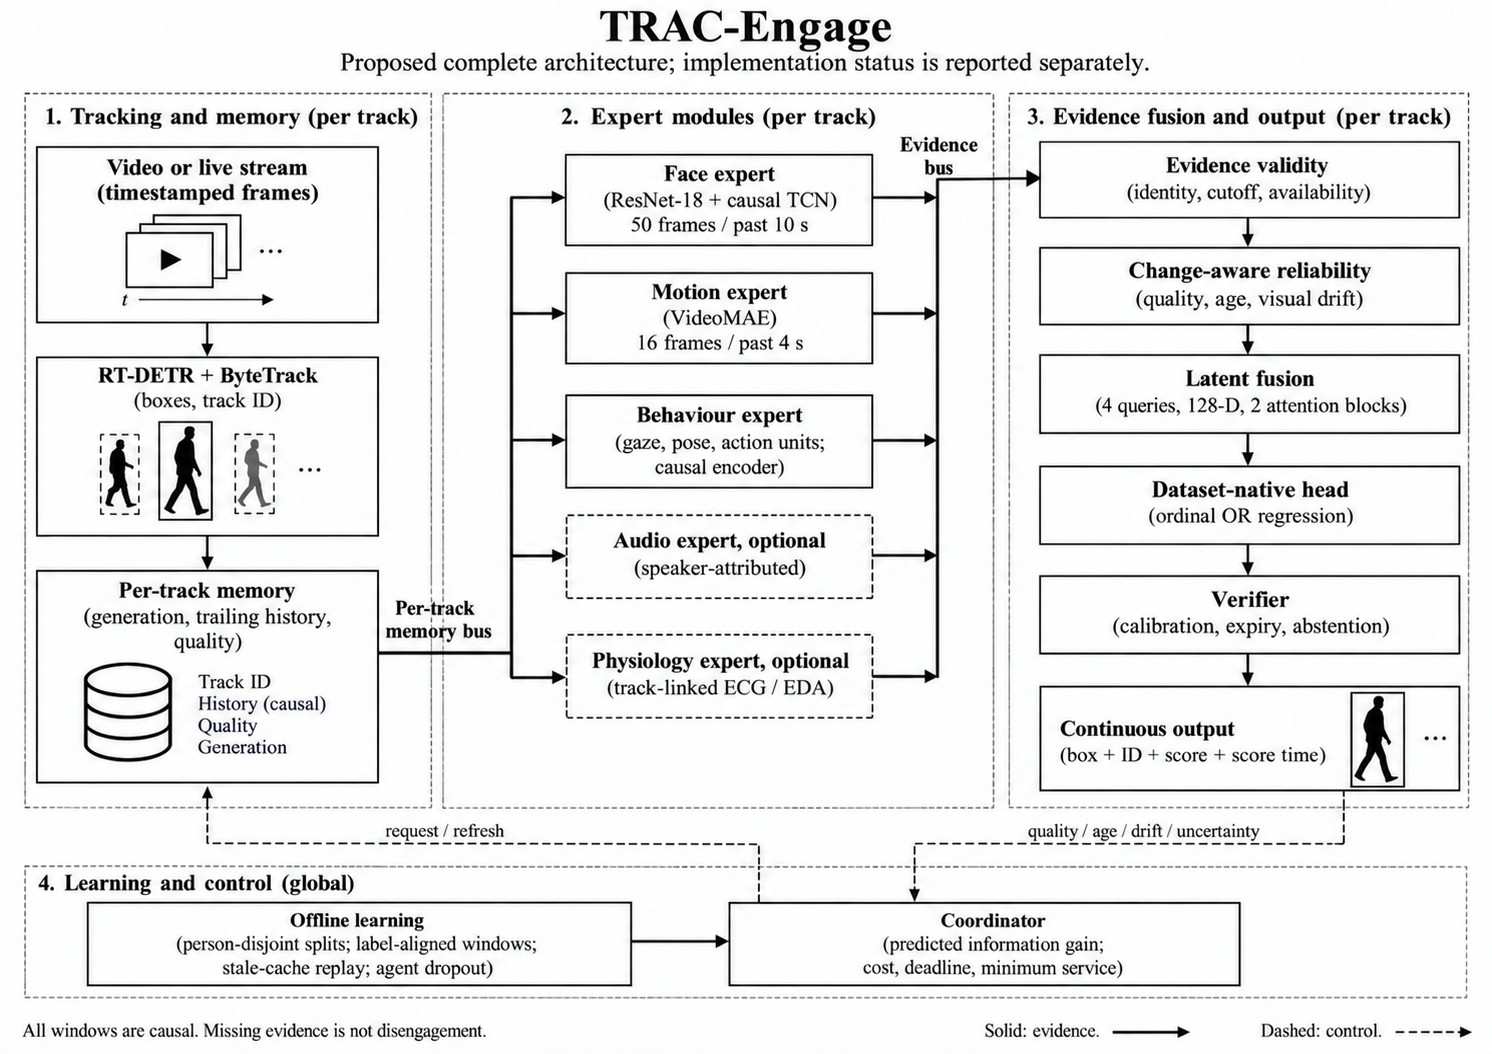
\includegraphics[width=\linewidth]{trac-engage-v2-architecture.png}
\caption{Complete proposed architecture. Solid arrows carry evidence/predictions; dashed arrows carry requests or feedback. The current code implements the temporal/fusion core and a single-face development path, not every extractor or the learned coordinator.}
\label{fig:map}
\end{figure}
\textbf{Read the diagram in four passes.} First follow video, tracking and memory. Next follow each specialist to the evidence bus. Then follow validity, reliability, fusion, head, verifier and output. Finally read the lower feedback loop: offline learning trains a coordinator that allocates future calls. Audio and physiology are optional inputs, not signals inferred from silent video.

\section{Bounding boxes, detection and tracking}
\subsection{Detection is a spatial prediction}
A box can be parameterized as $b=(x,y,w,h)$, with top-left position and size. A detector predicts boxes, categories and detection confidence. Intersection-over-union measures geometric agreement:
\begin{equation}
\operatorname{IoU}(A,B)=\frac{|A\cap B|}{|A\cup B|}.
\end{equation}
IoU is zero for disjoint boxes and one for identical boxes. It says nothing about engagement. A detector's confidence that a rectangle contains a person is also not engagement confidence.

\subsection{RT-DETR: set prediction with attention}
RT-DETR is the proposed person detector \cite{rtdetr}. A visual backbone creates feature maps; an encoder combines spatial scales; object queries attend to those features and predict a finite set of objects. Think of an object query as a learned slot asking, ``Which object should this slot describe?'' During detector training, predicted slots are matched to ground-truth objects with a one-to-one assignment and classification/localization losses. An engagement dataset need not retrain this detector from scratch. A pretrained detector may be frozen, but person-detection performance must still be measured for the target camera conditions.

\subsection{Why detection alone does not preserve people}
The order of detected boxes is arbitrary. Box 1 in frame $t$ need not represent box 1 in frame $t+1$. A tracker maintains a state, for example position, size and velocity, predicts its next location, then matches detections to predicted tracks. A simple assignment objective is
\begin{equation}
\min_{\pi}\sum_k C_{k,\pi(k)},\qquad
C_{kj}=1-\operatorname{IoU}(\hat b_{k,t},b_{j,t})+\text{gating penalties}.
\end{equation}
ByteTrack associates high-confidence detections first and uses lower-confidence detections to recover otherwise unmatched tracks \cite{bytetrack}. This can help through occlusion, but it does not eliminate identity switches. A track identifier is not biometric identity and should not be used to identify a person across unrelated recordings.

\subsection{Track generations and memory reset}
We attach a generation $g_k$ to a track's lifetime. On a suspected identity discontinuity or reinitialization, the generation increments and old evidence is invalidated. Otherwise a high-confidence score for person A could be displayed over person B. Memory is keyed by $(k,g_k)$ rather than by a reusable integer alone. Face-to-person association also needs spatial containment and temporal consistency, not simply the nearest face in one frame.

\textbf{Implemented limitation.} The local development path currently uses a unique frontal Haar face detector and an IoU continuity check. This is an inexpensive software scaffold, not RT-DETR, ByteTrack, landmark alignment or robust multi-person identity handling. It resets on absent or ambiguous faces. It must be replaced and tested before the complete architecture can be claimed.

\section{Embeddings, pretraining, freezing and fine-tuning}
An embedding extractor maps an image crop to a vector $z=f_\phi(I)\in\R^d$. The coordinates are learned features, not human-readable units such as ``attention''. A downstream head $g_\theta$ converts these features to the task output. Pretraining learns $\phi$ on another objective or dataset; task training learns an engagement-specific mapping.

\subsection{ResNet-18 from the CNN you already know}
Repeated convolutional blocks extract progressively larger visual patterns. A residual block uses
\begin{equation}
h_{l+1}=h_l+F_l(h_l;\phi_l),
\end{equation}
with a projection on the skip path when shape changes. The derivative contains an identity term: $\partial h_{l+1}/\partial h_l=I+\partial F_l/\partial h_l$. This improves optimization of deep feature extractors \cite{resnet}. Removing ResNet-18's original classifier leaves a 512-dimensional pooled representation. ImageNet pretraining gives useful visual structure, not a pretrained engagement measurement.

\subsection{Exactly which parameters are updated?}
For a frozen encoder, $\phi$ is held constant and only $\theta$ receives updates:
\begin{equation}
z_i=\operatorname{stopgrad}(f_\phi(I_i)),\quad
\theta\leftarrow\theta-\eta\nabla_\theta\ell(g_\theta(z_i),y_i).
\end{equation}
The current face extractor sets evaluation mode and disables gradients. This also avoids updating batch-normalization statistics. The trainable temporal projections, convolutions, fusion weights, learned queries and ordinal head still learn. Precomputing frozen embeddings makes CPU training practical, but consumes storage and prevents gradients from improving the encoder.

Fine-tuning unfreezes some or all of $\phi$, typically with a smaller learning rate than the head. It may adapt to subtle facial cues, but can overfit a small dataset. Choose freezing versus partial unfreezing on validation people, never on test people. Preprocessing must match the pretrained weights: channel order, crop construction, resizing and normalization all affect features. The same pipeline must be used at training and inference.

\section{Temporal evidence and causal convolution}
\subsection{Trailing windows}
A base decision uses 50 samples at 5 Hz, roughly ten seconds of observed history. Let $X=[z_1,\ldots,z_T]\in\R^{T\times512}$. A linear projection maps each $z_t$ to width $d=128$. A temporal convolution applies the same weights along time:
\begin{equation}
h'_t=\sigma\!\left(\sum_{j=0}^{K-1}W_j h_{t-j\delta}+b\right),
\end{equation}
where $\delta$ is dilation. Causality follows from using only indices at or before $t$ and padding on the left, not symmetrically. Dilation increases temporal reach without increasing the number of kernel weights.

\subsection{Receptive field versus whole-window support}
The implemented encoder has three residual blocks, each containing one kernel-three convolution, with dilations $1,2,4$. Its per-output receptive field is
\begin{equation}
R=1+(3-1)(1+2+4)=15\ \text{samples}.
\end{equation}
At 5 Hz those taps span 2.8 s from first to last sample. This is not a ten-second receptive field per output. We average all 50 causal outputs to summarize the complete history: $h=T^{-1}\sum_t h'_t$. Consequently the final window token can use the whole trailing window even though each intermediate output has local support. This distinction prevents an easy architecture-description error.

Layer normalization acts over feature channels at one time step. A normalization operation over the entire temporal axis could let future samples affect earlier outputs during training. The supplied causality test changes later inputs and verifies that earlier encoded states do not change. At inference, warm-up is required; padding an empty history and claiming a full-history estimate would be misleading.

\subsection{Relation to an RNN}
An RNN recursively compresses previous input into hidden state. A TCN uses a bounded stack of causal convolutions and can process training positions in parallel \cite{tcnfoundation}. Neither is automatically superior. RNN state reset and TCN window reset must both respect person changes. Temporal smoothing can reduce flicker but also delay true transitions, so transition delay must be evaluated separately from clip accuracy.

\section{The more expensive motion and behaviour specialists}
\subsection{VideoMAE}
Instead of treating each frame independently, a video Transformer divides a short clip into spatiotemporal patches or tubelets, projects them to tokens, adds positional information and applies attention. VideoMAE pretrains by hiding a large portion of these tokens and reconstructing missing visual content \cite{videomae}. A schematic pretraining loss is
\begin{equation}
\mathcal L_{\rm rec}=\frac1{|\mathcal M|}\sum_{j\in\mathcal M}
\|\hat x_j-x_j\|_2^2,
\end{equation}
where $\mathcal M$ indexes masked patches. The reconstruction decoder is not required for engagement inference. The pretrained encoder produces representations; an engagement-specific projection/head is learned afterwards.

Our proposal invokes this branch on 16 sampled frames from the previous four seconds when useful, rather than on every frame. Attention between those 16 frames is acceptable because all precede the decision time. Sampling later frames from the full video would invalidate a live-inference claim. The current repository exposes feature dimensions for this branch but does not yet integrate VideoMAE extraction or weights.

\subsection{Explicit facial and body behaviour}
Landmarks describe locations; head pose describes orientation; gaze estimates viewing direction; facial action units describe visible muscle-related movements. OpenFace is one established extraction toolkit \cite{openface}. A temporal encoder can learn how these measurements change over time. Their advantages are lower dimensionality and inspectability; disadvantages include measurement error, cultural/contextual confounding, occlusion and pose sensitivity.

The illustrative 35-dimensional behaviour interface is a configurable placeholder dimension, not a claim that OpenFace outputs exactly 35 numbers. An implementation must specify the selected columns, units, validity flags and train-fitted normalization. An off-camera gaze estimate cannot deterministically map to disengagement. Body pose or interaction context may resolve ambiguity, but must be tested through an ablation.

\section{Audio and physiology as genuine additional modalities}
\subsection{Audio}
An audio encoder can process waveform segments or time--frequency features. Prosody includes energy, pitch variation and timing; speech embeddings may add linguistic information. However a room microphone records mixtures of people. A per-person score requires speaker attribution or a declared group-level audio context. Unattributed room speech must not silently become evidence about every visible person.

\subsection{Physiology}
ECG records cardiac electrical activity; extracted beat intervals can describe heart-rate variability. EDA records changes in skin conductance related to sympathetic activity. Neither is engagement ground truth. Motion, temperature, physical exertion, medication and stress can confound interpretation. Processing requires signal-quality checks, artifact handling and windows appropriate to the feature. A stable HRV estimate can need much longer support than a four-second video clip; it should enter as a slower contextual token, not as a fabricated instantaneous measurement.

The future physiological branch uses modality-specific temporal encoders and carries participant linkage and acquisition timestamps. Sensor units must be preserved. A missing sensor is masked, not replaced by a zero that looks like a real physiological value. Meridian can supply these recordings later, but sensor availability alone does not supply labels, synchronized clocks or a lawful person-to-track mapping.

\subsection{Why intermediate fusion?}
\begin{itemize}
\item \textbf{Early fusion:} concatenate raw/aligned features before learning. Simple, but units, rates and missing streams need careful treatment.
\item \textbf{Late fusion:} combine independently predicted probabilities. Modular, but interactions between evidence streams are restricted.
\item \textbf{Intermediate fusion:} each encoder learns a representation, then a joint module exchanges information before prediction. This is our chosen design.
\end{itemize}
An ensemble of three visual encoders remains video-only multi-view inference. It becomes multimodal when independent sensing channels such as audio or ECG join. Multi-agent and multimodal are separate concepts: many agents can inspect one modality, while one network can fuse several modalities.

\section{Evidence contracts: who, when and how reliable?}
For expert $m$ and track $k$, a message contains
\begin{equation}
e_{km}=(k,g_k,m,[a,b],t_{\rm received},z,q,\nu),
\end{equation}
where $[a,b]$ is the observation support, $z$ the embedding, $q$ estimated quality and $\nu$ the model version. Event time $b$ is not the same as arrival time. Network delay must not make old evidence appear current.

At decision time $t$, a validity predicate can require matching generation, $a\leq b\leq t$, arrival by $t$, finite features, acceptable quality and $t-b\leq T_m$. These checks are deterministic software, not learned psychological judgments. Invalid evidence is removed before attention. Keeping the checks outside the neural network makes their behaviour auditable.

\subsection{Age and drift reliability}
Age alone misses rapid changes: a one-second-old token may be fine in a stable shot but unreliable just after a person turns away. A cheap current embedding $u_t$ provides a change measure relative to the cached expert's observation time $b$:
\begin{equation}
\delta_{km}=\max\!\left(0,1-\frac{u_t^\top u_b}{\|u_t\|\|u_b\|}\right),\qquad
r_{km}=v_{km}q_{km}\exp[-(t-b)/\tau_m-\beta\delta_{km}].
\end{equation}
Here $v\in\{0,1\}$ is hard validity. This is a proposed reliability signal, not proof that engagement changed. Lighting changes can also move embeddings. It therefore needs comparison with age-only weighting at equal coverage and cost. Wrong-person evidence is never made acceptable merely by assigning a small positive reliability.

\section{Latent attention fusion, step by step}
Suppose $M$ specialists each produce a 128-dimensional token. Add a learned modality identifier, stack into $H\in\R^{M\times128}$ and introduce four learned query vectors $Q_0\in\R^{4\times128}$. These queries are trainable parameters shared across examples, not natural-language prompts. They provide a small common workspace.

One attention head computes
\begin{equation}
A=\softmax\left(\frac{(QW_Q)(HW_K)^\top}{\sqrt{d_h}}+B\right),
\qquad Z=A(HW_V),
\end{equation}
where $B_{jm}=\log r_m$ for valid tokens and $-\infty$ for invalid ones. The softmax makes nonnegative weights summing to one over available evidence. Adding $\log r_m$ multiplies its unnormalized attention weight by reliability. Learned compatibility and measured reliability thus both influence exchange.

Four heads run in parallel; their outputs are concatenated and projected. Residual addition, layer normalization and a feed-forward network give the familiar Transformer pattern. We apply two cross-attention blocks and average the four final queries. The latent-bottleneck idea is motivated by prior multimodal fusion research \cite{mbt}; our exact small-query configuration is a design choice requiring validation, not a published optimal setting.

\subsection{All-missing evidence and numerical safety}
Softmax over only $-\infty$ values is undefined. The implementation inserts a neutral sentinel for this numerical case and returns \texttt{usable=false}. The internal numerical output must never be displayed. NaNs, future ages and expired tokens are masked. A masked-branch invariance test changes an unavailable branch and verifies that the prediction remains unchanged.

\subsection{What is actually learned?}
Parameters include each expert's projection/convolution weights, modality identifiers, latent queries, $W_Q,W_K,W_V$, attention output projections, feed-forward layers, layer-normalization gains/offsets and the prediction head. Quality, availability, ages and track IDs are input metadata or rules, not magically learned labels. The current code uses supplied drift values; it does not automatically build stale-cache replay trajectories.

\section{Ordinal prediction and the meaning of the score}
For $K$ ordered levels, independent softmax classification ignores that confusing adjacent levels is less severe than confusing extremes. We instead predict cumulative probabilities $o_j=P(y>j\mid x)$ for $j=0,\ldots,K-2$. Let $a=w^\top h+b$ be a learned location and define ordered cutpoints
\begin{equation}
\theta_0=c,\quad \theta_j=c+\sum_{i=1}^j\softplus(g_i),\quad
o_j=\sigmoid(a-\theta_j).
\end{equation}
Since $\softplus(g)=\log(1+e^g)>0$, cutpoints increase and cumulative probabilities decrease. This follows established rank-consistent ordinal modelling principles \cite{coral}. It is not our novelty.

Class probabilities are $p_0=1-o_0$, $p_j=o_{j-1}-o_j$ for interior classes, and $p_{K-1}=o_{K-2}$. They are nonnegative and telescope to one. For targets $t_j=\ind[y>j]$, the cumulative loss is
\begin{equation}
\mathcal L_{\rm ord}=-\frac1{K-1}\sum_{j=0}^{K-2}
\big[t_j\log o_j+(1-t_j)\log(1-o_j)\big].
\end{equation}
For a logit $\ell_j=a-\theta_j$, the derivative of its binary loss is $o_j-t_j$. Gradients propagate through the head, fusion and temporal encoders; they stop at a frozen image extractor.

The index is the normalized expected ordinal level:
\begin{equation}
s=\frac{100}{K-1}\sum_{j=0}^{K-1}jp_j
=\frac{100}{K-1}\sum_{j=0}^{K-2}o_j.
\end{equation}
For four levels and $o=(0.9,0.6,0.2)$, $p=(0.1,0.3,0.4,0.2)$ and $s=56.7$. This is not ``56.7\% attentive'', a clinical measure, or a calibrated probability of engagement. Expected ordinal error and argmax classification accuracy can disagree; both should be reported.

Continuous-label corpora require a separate head and objective. Concordance correlation is
\begin{equation}
\mathrm{CCC}=\frac{2\operatorname{cov}(y,\hat y)}{sigma_y^2+\sigma_{\hat y}^2+(\mu_y-\mu_{\hat y})^2},
\end{equation}
which penalizes location/scale mismatch as well as lack of correlation. A loss can combine $1-\mathrm{CCC}$ with MAE. The current implementation contains the ordinal head only; continuous regression remains a planned extension.

\section{What makes a specialist an agent?}
A neural encoder is a function. An agent is a stateful entity with observations, actions, memory and an objective. In this proposal, specialists expose operations such as refresh evidence, return cached evidence or report failure. A coordinator chooses operations under resource constraints. There is no requirement for language generation, a chat interface, separate operating-system processes or an LLM.

\subsection{Decision problem}
The coordinator's state $s_t$ includes evidence age/quality, disagreement, drift, queue load and remaining budget. Its action can request an expert, keep a valid cache, defer or abstain. A sequential formulation is
\begin{equation}
\pi^*=\arg\max_\pi\E_\pi\sum_t\gamma^t
[-\ell(\hat y_t,y_t)-\lambda c(a_t)-\mu d(a_t)],
\end{equation}
where $c$ measures resource cost and $d$ deadline violations. Engagement labels are unavailable during normal live use, so the reward cannot be observed directly online. Policy learning must use labelled training replays or a carefully justified proxy.

\subsection{Value of information rather than expert voting}
For a candidate refresh, define the value of information as expected loss reduction after acquiring it:
\begin{equation}
U_{km}=\E[\ell(\hat y_{\rm cached},y)-\ell(\hat y_{\rm refreshed(m)},y)\mid s_t].
\end{equation}
Train a predictor $\hat U_\psi(s_t,m)$ from out-of-fold teacher replays. Out-of-fold means the teacher predicting a training person's examples was fitted without that person's fold. Otherwise unrealistically accurate training predictions can distort the scheduler's utility targets.

Selection is a constrained allocation problem:
\begin{equation}
\max_{z_{km}\in\{0,1\}}\sum_{km}z_{km}\hat U_{km},\qquad
\sum_{km}z_{km}c_{km}\leq B_t.
\end{equation}
Greedy utility/cost ranking is an inexpensive baseline, not generally the exact knapsack optimum. Add minimum-service or maximum-refresh-gap constraints so one easy or prominent person does not absorb the budget. When the budget cannot satisfy all obligations, surface degraded service rather than silently claiming healthy coverage.

\subsection{Multi-agent research does not guarantee novelty}
Adaptive frame selection, agent interaction and multimodal fusion already exist \cite{adaframe,edf}. The proposed research contribution is the joint treatment of person identity, evidence expiry, drift, per-track service and learned acquisition value. Run exactly the same encoders with always-on, periodic, random and uncertainty-based schedules. If a simple schedule matches the accuracy--latency frontier, the extra agent machinery is not justified. Running agents in separate processes is an implementation choice, not evidence of an algorithmic improvement.

\section{The proposed additional novelty: stale-cache replay}
Training fusion only with simultaneous fresh tokens creates a mismatch: the deployed scheduler usually supplies a mixture of fresh and cached tokens. The proposed extension replays actual earlier tokens from the same track generation with their true support and age. It does not shuffle arbitrary people together or relabel old observations as current.

For a training decision at $t$, sample legal cache times $b_m\leq t$, construct $\tilde z_m=z_m(b_m)$ and feed $(\tilde z_m,q_m,t-b_m,\delta_m)$. The target remains the annotation appropriate to the decision/support protocol. The loss can include ordinary supervised loss and, only when justified, consistency with a fresh-evidence teacher:
\begin{equation}
\mathcal L=\mathcal L_{\rm ord}(p_{\rm replay},y_t)
+\lambda\,\operatorname{KL}(p_{\rm teacher}\Vert p_{\rm replay}).
\end{equation}
The teacher must be reliable and out-of-fold; forcing agreement near genuine transitions can be harmful. Start with supervised replay and treat distillation as a separate ablation. Replay cannot teach dense transition response from clip labels that contain no transition annotations.

The decisive factorial experiment crosses two choices: age-only versus age-and-drift reliability, and fresh-only versus replay training. Match encoders, compute budget, folds and coverage. Report stale-score duration, transition delay, ordinal error and calls. An improvement only from abstaining more often is not a successful result. This experiment is proposed, not performed in the current artifacts.

\section{Calibration, abstention and the verifier}
Confidence can be high even when a prediction is wrong. Temperature scaling uses held-out calibration people to choose $T>0$, then transforms logits $\ell/T$ \cite{guo}. In the ordinal head this preserves cutpoint order. Fit $T$ by class-probability negative log-likelihood on calibration data only. Calibration data must also reflect the deployed scheduling policy. A calibrated in-domain model can still fail under domain shift.

Abstention adds a reject option: the system can decline to provide a score when evidence is insufficient \cite{selective}. A verifier checks identity, time, evidence support, expiry and the calibrated acceptance rule. Its outputs include warming-up, usable, stale and insufficient-evidence states. Rejection is not class zero.

For an acceptance threshold $\alpha$,
\begin{equation}
\operatorname{coverage}(\alpha)=\frac{\sum_i\ind[c_i\geq\alpha]}N,\quad
\operatorname{risk}(\alpha)=\frac{\sum_i\ell_i\ind[c_i\geq\alpha]}{\sum_i\ind[c_i\geq\alpha]}.
\end{equation}
Report the risk--coverage curve and the total visible-person time. Reporting accuracy only on accepted easy faces conceals service failure. Hard metadata checks are implemented; a validated predictive rejection policy and production calibration are not yet available.

\section{Training, tuning and defensible experiments}
\subsection{Dataset choice and leakage prevention}
DAiSEE provides a four-level webcam benchmark with an official research-use access procedure \cite{daisee}. DIPSER, also named DIPSEER in the release, supplies in-person engagement annotations under CC BY 4.0; its complete official listing is about 668 GB \cite{dipser}. Neither was retrieved as a ready-to-train corpus in this work. Instead, the authors' public CMOSE feature release was downloaded and checksum-verified under CC BY-SA 4.0 \cite{cmose}. It permits a small real-label CPU experiment without downloading raw video. Emotion clips supplied to Meridian are not substitutes for engagement labels.

The audited CMOSE subset has 11,902 usable clips after excluding 295 empty visual embeddings. Each clip supplies a 1024-dimensional I3D video embedding, 768-dimensional BERT transcript embedding and six acoustic summary values. A clip embedding summarizes an entire interval, not a frame. Treating it as one temporal token permits fusion testing but says nothing about within-clip transitions, causal extraction latency or tracking. This distinction is the difference between testing a component and validating a system.

The fixed split holds out whole coaching sessions: six sessions train, session 15 validates, session 16 calibrates, and session 10 tests. Counts are 8,806, 709, 734 and 1,653 respectively. Person identifiers are session-scoped; biological identity across sessions is not known. We therefore claim session-disjoint, not verified globally subject-disjoint, evaluation. Feature means and standard deviations are fitted on training clips only. The single test session and very rare lowest-engagement class limit conclusions.

Create participant-disjoint training, validation, calibration and test partitions. Keep overlapping windows and repeated sessions from a person together. In interaction data, connected groups may also need grouping to avoid the same partners/scene leaking across splits. Fit normalization on training only; log annotation scales, original time support, licences and exclusions. A manifest hash catches accidental split-file changes, but does not verify that claimed identities or labels are correct.

\subsection{Optimization and staged learning}
The initial implementation trains temporal/fusion/head parameters with AdamW, learning rate $3\times10^{-4}$, weight decay $10^{-4}$, batch size 16 and gradient-norm clipping at 1. These are starting settings, not tuned engagement results. Early stopping uses validation ordinal MAE. Optional-agent dropout teaches fusion to tolerate missing branches, while preserving the base path.

The intended full training order is: train individual experts; train masked fusion; learn utility from out-of-fold evidence; add legal stale-cache replay; fit calibration under the selected policy; then evaluate the locked test set. Unfreezing encoders or changing losses is a new configuration, not a reason to reuse the test set for tuning. The bounded CMOSE pilot compares visual-only mean fusion, multimodal mean fusion and multimodal latent attention. It uses width 32, batch 128, at most ten epochs and patience four. Two learning rates are selected using validation MAE at seed 17, then seeds 31 and 53 repeat each selected configuration. Only afterward are temperature and held-out test metrics computed. This is not training the full agentic architecture.

\subsection{Metrics and scale}
Macro-F1 weighs classes equally; balanced accuracy averages class recalls; ordinal MAE measures distance between expected level and label; NLL and Brier score assess predictive distributions. For $K$ classes,
\begin{equation}
\mathrm{Brier}=\frac1N\sum_i\sum_{j=0}^{K-1}(p_{ij}-\ind[y_i=j])^2.
\end{equation}
Also measure detection AP, track IDF1, identity switches, wrong-person score duration, score age, latency percentiles and throughput as people increase. These are separate from engagement accuracy. Use participant-cluster bootstrap intervals: resample whole participants, not highly correlated adjacent frames. Report missing classes and rejected windows.

The target of 1--8 people in a 720p stream with one decision/s is a proposed engineering target, not measured capacity. The current CPU smoke test on tiny embeddings says nothing about VideoMAE, multi-person tracking, camera decoding or full-system latency. GPU availability and model compatibility must be established independently.

\section{Implementation audit and what the experiments currently show}
The repository now contains a PyTorch temporal/fusion/ordinal core, evidence checks, split-validated NPZ training, a validation-only sweep, calibration/evaluation commands, a frozen face-feature extractor and a guarded local inference scaffold. It does not yet contain the complete multi-person detector/tracker integration, all specialist extractors, a trained utility policy or stale-cache replay. The application portal is unchanged.

The first engineering run used generated arrays with four artificial classes, 64 training examples and 24 validation examples, not human faces. Twelve CPU epochs reduced cumulative training loss from 0.3472 to 0.2183. This establishes that gradients, optimizer updates and checkpoint writing execute. A separate synthetic calibration/test pass exercises probability metrics. None of these numbers establishes engagement recognition, generalization, novelty or production quality. Synthetic checkpoints are explicitly rejected by the human-video inference command.

Tests cover ordered normalized probabilities, all-missing inputs, masked-branch invariance, temporal causality, identity/time/expiry rejection, drift penalties, non-finite features, gradient updates, budget limits, split leakage and synthetic-checkpoint rejection. Passing a test proves only its specific invariant. CMOSE feature-model checkpoints are separate from the 512-dimensional ResNet face pipeline: substituting I3D-trained weights into that pipeline is invalid and rejected. Camera/live inference still requires dedicated integration and validation. The research paper and saved experiment logs report the public-data pilot separately from these software checks.

\subsection{How to read the source}
\textbf{Reading the real-data result.} The CMOSE pilot completed 12 training runs and evaluated three selected configurations across three seeds. After calibration, visual mean, multimodal mean and multimodal latent fusion obtained mean macro-F1 of 24.76\%, 25.36\% and 25.39\%, respectively. Their ordinal MAEs were 0.691, 0.647 and 0.662 on the 0--3 label scale. A training-majority constant achieved 19.16\% macro-F1 but a better MAE of 0.415. Thus one metric improves while another worsens: there is no basis for claiming a generally better detector. Uncalibrated model MAEs were lower (0.500, 0.477, 0.464), demonstrating that NLL-fitted temperature need not improve ordinal error under session shift. These are feature-level results, not tests of the full diagram. The research paper records the complete table, split limitations and seed variation.

\begin{itemize}
\item \texttt{trac/model.py}: trainable temporal encoders, reliability weighting, attention and ordinal head.
\item \texttt{trac/contracts.py}: deterministic evidence validation and a simple budget allocator.
\item \texttt{trac/data.py}, \texttt{prepare.py}: provenance/split checks and development face features.
\item \texttt{train.py}, \texttt{sweep.py}, \texttt{evaluate.py}: optimization, validation selection and held-out evaluation.
\item \texttt{infer.py}: local research-only single-face pipeline; not the complete proposed detector.
\end{itemize}
Do not set a flag to manufacture a production claim. Required evidence includes real labels, external-domain evaluation, calibrated coverage, tracker validation, matched-budget ablations, privacy review and operational recovery tests. There is no deployed service or production checkpoint in this deliverable.

\section{Worked reasoning exercises}
\textbf{1. Stale versus fresh.} Two tokens have equal quality $q=0.8$, decay $\tau=4$ s and no drift. At ages 0 and 4 s their reliability is $0.8$ and $0.8e^{-1}\approx0.294$. Attention can still learn that the older token is useful, but it begins with a lower prior weight. If its generation is wrong, reliability becomes exactly zero regardless of age.

\textbf{2. Causality.} Predicting engagement at 10 s from a clip containing frames through 12 s is not causal. Predicting at 12 s from that same clip is causal if all frames have arrived by the decision deadline. Event time and delivery time both matter.

\textbf{3. Utility.} Expert A costs 20 ms and is predicted to reduce loss by 0.04; expert B costs 60 ms and reduces it by 0.06. Their ratios are 0.002 and 0.001 loss/ms. A greedy allocator prefers A, but minimum service or combinations of jobs can change the optimal allocation. Predicted utility must itself be tested.

\textbf{4. Missingness.} A zero-valued ECG feature could be a valid standardized average, a disconnected lead or a padding value. Without a validity mask the network cannot distinguish these cases. The interface therefore carries both the numerical feature and its availability/quality metadata.

\textbf{5. Novelty test.} Suppose replay reduces MAE but doubles abstention. This is not yet a better detector. Compare risk at the same coverage and compare total stale/wrong-person exposure. The system's purpose is reliable continuous service, not an attractive isolated accuracy number.

{\small
\begin{thebibliography}{99}
\bibitem{resnet} K. He et al., ``Deep residual learning for image recognition,'' CVPR, 2016. \url{https://arxiv.org/abs/1512.03385}.
\bibitem{tcnfoundation} S. Bai, J. Z. Kolter and V. Koltun, ``An empirical evaluation of generic convolutional and recurrent networks for sequence modeling,'' 2018. \url{https://arxiv.org/abs/1803.01271}.
\bibitem{videomae} Z. Tong et al., ``VideoMAE: Masked autoencoders are data-efficient learners for self-supervised video pre-training,'' NeurIPS, 2022. \url{https://arxiv.org/abs/2203.12602}.
\bibitem{rtdetr} Y. Zhao et al., ``DETRs beat YOLOs on real-time object detection,'' CVPR, 2024. \url{https://arxiv.org/abs/2304.08069}.
\bibitem{bytetrack} Y. Zhang et al., ``ByteTrack: Multi-object tracking by associating every detection box,'' ECCV, 2022. \url{https://arxiv.org/abs/2110.06864}.
\bibitem{openface} T. Baltru\v{s}aitis et al., ``OpenFace 2.0: Facial behavior analysis toolkit,'' IEEE FG, 2018. \url{https://doi.org/10.1109/FG.2018.00019}.
\bibitem{mbt} A. Nagrani et al., ``Attention bottlenecks for multimodal fusion,'' NeurIPS, 2021. \url{https://arxiv.org/abs/2107.00135}.
\bibitem{coral} W. Cao, V. Mirjalili and S. Raschka, ``Rank consistent ordinal regression for neural networks with application to age estimation,'' Pattern Recognition Letters, 2020. \url{https://arxiv.org/abs/1901.07884}.
\bibitem{adaframe} Z. Wu et al., ``AdaFrame: Adaptive frame selection for fast video recognition,'' CVPR, 2019. \url{https://arxiv.org/abs/1811.12432}.
\bibitem{edf} M. Sun and S. Feng, ``Deep learning for student engagement analysis in educational psychology,'' Frontiers in Psychology, 2026. \url{https://doi.org/10.3389/fpsyg.2026.1764399}.
\bibitem{guo} C. Guo et al., ``On calibration of modern neural networks,'' ICML, 2017. \url{https://proceedings.mlr.press/v70/guo17a.html}.
\bibitem{selective} Y. Geifman and R. El-Yaniv, ``SelectiveNet: A deep neural network with an integrated reject option,'' ICML, 2019. \url{https://proceedings.mlr.press/v97/geifman19a.html}.
\bibitem{daisee} A. Gupta et al., ``DAiSEE: Towards user engagement recognition in the wild,'' 2016. \url{https://arxiv.org/abs/1609.01885}. Official access: \url{https://people.iith.ac.in/vineethnb/resources/daisee/}.
\bibitem{dipser} L. M\'arquez-Carpintero et al., DIPSER/DIPSEER dataset, version 5, Science Data Bank, 2025. \url{https://doi.org/10.57760/sciencedb.11541}.
\bibitem{cmose} C.-H. Wu et al., ``CMOSE: Comprehensive multi-modality online student engagement dataset with high-quality labels,'' CVPR Workshops, 2024, pp. 4636--4645. \url{https://jasonwuchi.github.io/CMOSE/}. Public features: \url{https://huggingface.co/datasets/cwuau/CMOSE}.
\end{thebibliography}
}
\end{document}
